\begin{chapter}{Some examples}
After introducing a method to produce a QP associated to an arbitrary polygonal subdivision of a surface, a natural question arises: is the associated Jacobian algebra always finite-dimensional? As shown in \cite{Lad12}, this is indeed the case for triangulations of closed surfaces. In this section, we will show that this is not true for arbitrary subdivisions. In fact, we will produce examples of both finite and infinite-dimensional algebras arising from subdivisions of closed surfaces of every genus.
\begin{section}{A family of finite-dimensional examples}

We start by showing that surfaces of any genus admit a particular decomposition into disjoint disks.

A \emph{loop} $f$ on a surface $\Sigma$ is a smooth embedding $f:S^1\to \Sigma$. We will identify a loop with its image on $\Sigma$. A \emph{handle} is a torus with a disk removed. We recall that a surface of genus $g>0$ can be obtained starting with a disk with $g-1$ holes and gluing handles along each hole and the boundary of the disk. \textcolor{red}{[citation needed]}

\begin{figure}[h]
\centering
	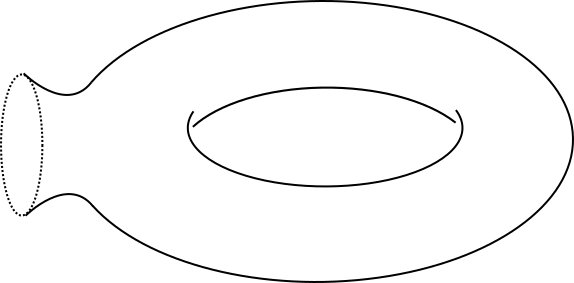
\includegraphics[width=0.5\textwidth]{handle.png}
\caption{A handle.}
\end{figure}

\begin{prop} Let $\Sigma$ be a surface of genus $g$. There exist finite families $\{r_i\}$ and $\{b_j\}$ of loops on $\Sigma$ such that:
\begin{enumerate}
\item Two loops in the same family are disjoint.
\item Any point of the surface belongs to at most two loops.
\item The loops divide the surface into a disjoint family of regions, each of them a disk (up to homeomorphism).
\end{enumerate}
\end{prop}

\begin{proof} We give an explicit construction of such families.

The case in which $g=0$ (the sphere) is easily dealt with by choosing a single loop $r_1$ as the equator, since both hemispheres are homeomorphic to a disk and the other conditions are vacuously true.

For the cases in which $g>0$, we will make use of the handle decomposition we mentioned previously. We will draw a handle as a square (with opposite edges identified) having a gray hole in its center. Consider the following configuration:

\begin{figure}[h]
\[
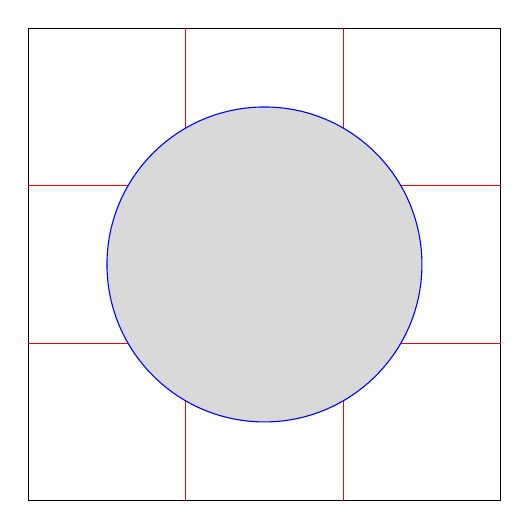
\begin{tikzpicture}
\draw (0,0) node[minimum size=6cm,draw] {};

\fill [black,opacity=.15] circle (2cm);

\draw[red] (-3,1) -- (-1.73,1);
\draw[red] (-3,-1) -- (-1.73,-1);

\draw[red] (3,1) -- (1.73,1);
\draw[red] (3,-1) -- (1.73,-1);

\draw[red] (1,-3) -- (1,-1.73);
\draw[red] (-1,-3) -- (-1,-1.73);

\draw[red] (1,3) -- (1,1.73);
\draw[red] (-1,3) -- (-1,1.73);

\draw[blue] (0,0) circle (2cm);
\end{tikzpicture}
\]
\end{figure}

We first deal with the case in which $g=1$. If we glue such a handle to the boundary of the following disk, we obtain a torus with a single red loop $r_1$ and a single blue loop $b_1$:

\begin{figure}[h]
\label{divided-handle}
\[
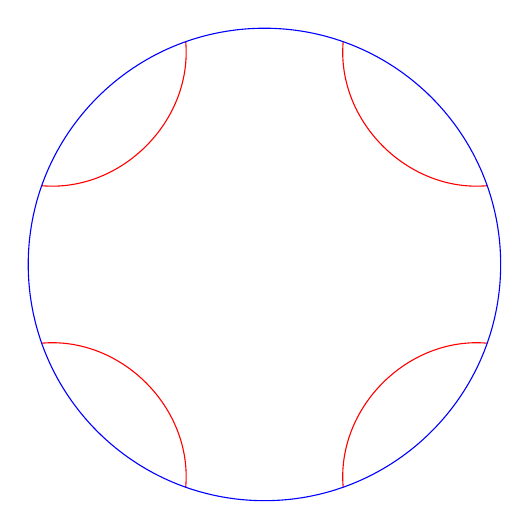
\begin{tikzpicture}

\draw[red] (-2.83,1) to [bend right=50] (-1,2.83);
\draw[red] (2.83,1) to [bend left=50] (1,2.83);
\draw[red] (2.83,-1) to [bend right=50] (1,-2.83);
\draw[red] (-2.83,-1) to [bend left=50] (-1,-2.83);

\draw[blue] (0,0) circle (3cm);
\end{tikzpicture}
\]
\end{figure}

Once again, the intersection conditions are vacuous. Finally, we observe that the blue loop cuts the torus into a disk and a handle, so one can check condition $3$ in both objects separately. One sees at once that the disk gets cut up into 5 smaller disks, while the handle is divided into $3$ disks, as we wanted.

\marginpar{el numero de ref deberia salir arriba}

While the solution to the case $g=1$ may be easier to draw directly on a square instead of considering a handle decomposition, the latter helps to illustrate the general case, which we now consider. For the case $g>1$, we regard our surface as a disk with $g-1$ holes, with a handle divided as in \ref{divided-handle} attached to its boundary and to each of its holes. We now exemplify the configuration on the \textcolor{red}{holed} disk for $g=4$:

\begin{figure}[h]
\[
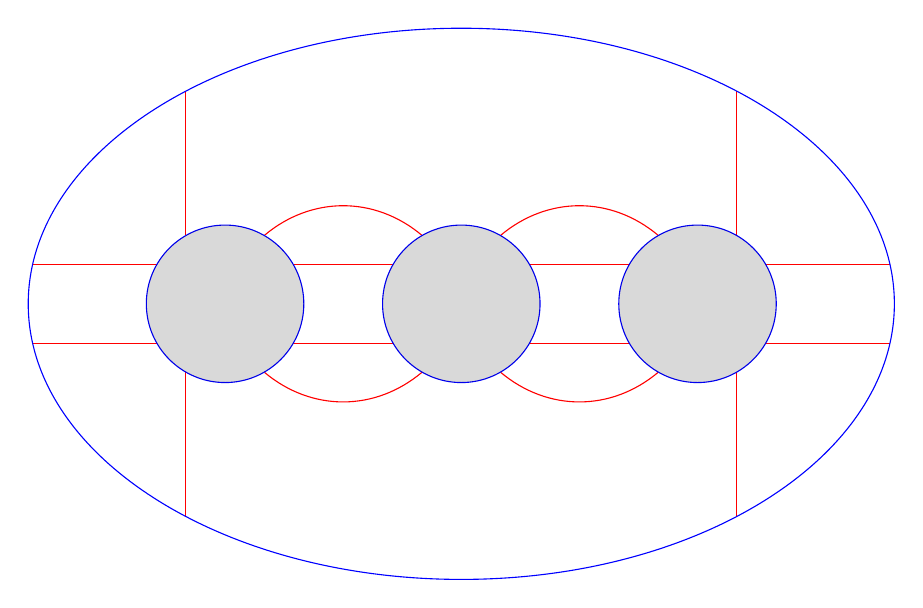
\begin{tikzpicture}
\draw[red] (-5.44, 0.5) -- (-3.87, 0.5);
\draw[red] (-5.44, -0.5) -- (-3.87, -0.5);
\draw[red] (5.44, 0.5) -- (3.87, 0.5);
\draw[red] (5.44, -0.5) -- (3.87, -0.5);

\draw[red] (-3.5,0.87) -- (-3.5,2.7);
\draw[red] (-3.5,-0.87) -- (-3.5,-2.7);
\draw[red] (3.5,0.87) -- (3.5,2.7);
\draw[red] (3.5,-0.87) -- (3.5,-2.7);

\draw[red] (-2.137, 0.5) -- (-0.863, 0.5);
\draw[red] (-2.137, -0.5) -- (-0.863, -0.5);
\draw[red] (2.137, 0.5) -- (0.863, 0.5);
\draw[red] (2.137, -0.5) -- (0.863, -0.5);

\draw[red] (-2.5,0.87) to [bend left=40] (-0.5,0.87);
\draw[red] (2.5,0.87) to [bend right=40] (0.5,0.87);
\draw[red] (-2.5,-0.87) to [bend right=40] (-0.5,-0.87);
\draw[red] (2.5,-0.87) to [bend left=40] (0.5,-0.87);

\draw[blue] (0,0) ellipse (5.5cm and 3.5cm);
\draw[blue] (0,0) circle (1cm);
\draw[blue] (-3,0) circle (1cm);
\draw[blue] (3,0) circle (1cm);
\fill [black,opacity=.15] (-3,0) circle (1cm);
\fill [black,opacity=.15] (0,0) circle (1cm);
\fill [black,opacity=.15] (3,0) circle (1cm);
\end{tikzpicture}
\]
\end{figure}

The following is an outline for the construction of the previous figure for general $g$:
\begin{enumerate}
\item Place the $g-1$ holes in a straight line inside the disk.
\item Connect the boundary of the left and rightmost holes to the boundary of the disk using 4 red arcs, mimicking the figure.
\item Cycle through the holes from left to right. If the current hole has a neighboring hole to its right, draw 4 red arcs connecting them.
\end{enumerate}

Notice that after gluing the handles, both the red and the blue arcs are now loops. We now consider the families $\{r_i\}$ and $\{b_j\}$, consisting of the red and blue loops respectively. Inspecting the figures, we see that conditions 1 and 2 are both satisfied. Finally, it remains to check condition 3. Since we have already seen that each handle is split up into disks, it suffices to check this for the \textcolor{red}{holed} disk, and once again this is easily seen from the drawing.
\end{proof}

A \emph{band} on a surface $\Sigma$ is a finite sequence $\{C_1, \dots, C_n\}$, where each $S_i$ is a quadrilateral on $\Sigma$ subdivided by one of its main diagonals, arranged as in one of the following two figures:

\[
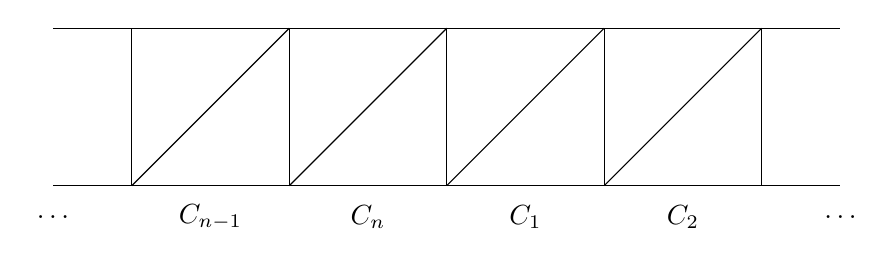
\begin{tikzpicture}
\draw (-5,1) -- (5,1);
\draw (-5,-1) -- (5,-1);

\foreach \x in {-4,-2,...,4}
\draw (\x,1) -- (\x,-1);

\foreach \x in {-4,-2,...,2}
\draw (\x,-1) -- (\x+2, 1);

\node at (-5,-1.4) {$\dots$};
\node at (-3,-1.4) {$C_{n-1}$};
\node at (-1,-1.4) {$C_{n}$};
\node at (1,-1.4) {$C_{1}$};
\node at (3,-1.4) {$C_{2}$};
\node at (5,-1.4) {$\dots$};
\end{tikzpicture}
\]

\[
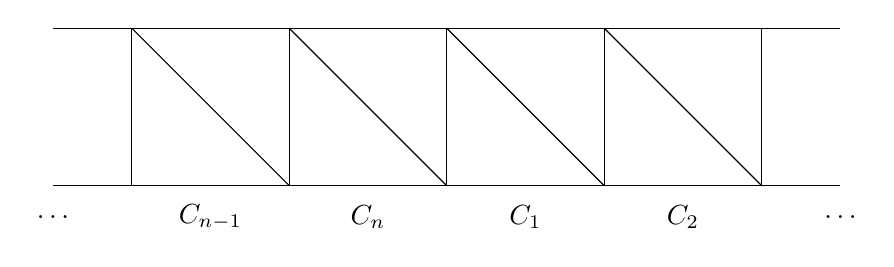
\begin{tikzpicture}
\draw (-5,1) -- (5,1);
\draw (-5,-1) -- (5,-1);

\foreach \x in {-4,-2,...,4}
\draw (\x,1) -- (\x,-1);

\foreach \x in {-4,-2,...,2}
\draw (\x,1) -- (\x+2, -1);

\node at (-5,-1.4) {$\dots$};
\node at (-3,-1.4) {$C_{n-1}$};
\node at (-1,-1.4) {$C_{n}$};
\node at (1,-1.4) {$C_{1}$};
\node at (3,-1.4) {$C_{2}$};
\node at (5,-1.4) {$\dots$};
\end{tikzpicture}
\]

Notice that in both cases the choice of diagonal is consistent throughout the band. We will say a band is \emph{positively oriented} if it is arranged as in the first figure and \emph{negatively oriented} otherwise. We require that the only adjacency relations between quadrilaterals in a band are the ones expressed by the figures, so in particular bands have well-defined top and bottom sides.
\end{section}
\end{chapter}